\section{Pillar 2: Language as Deliberative Feedback}%
\label{sec:pillar2}

\begin{figure}[!t]
     \centering    
    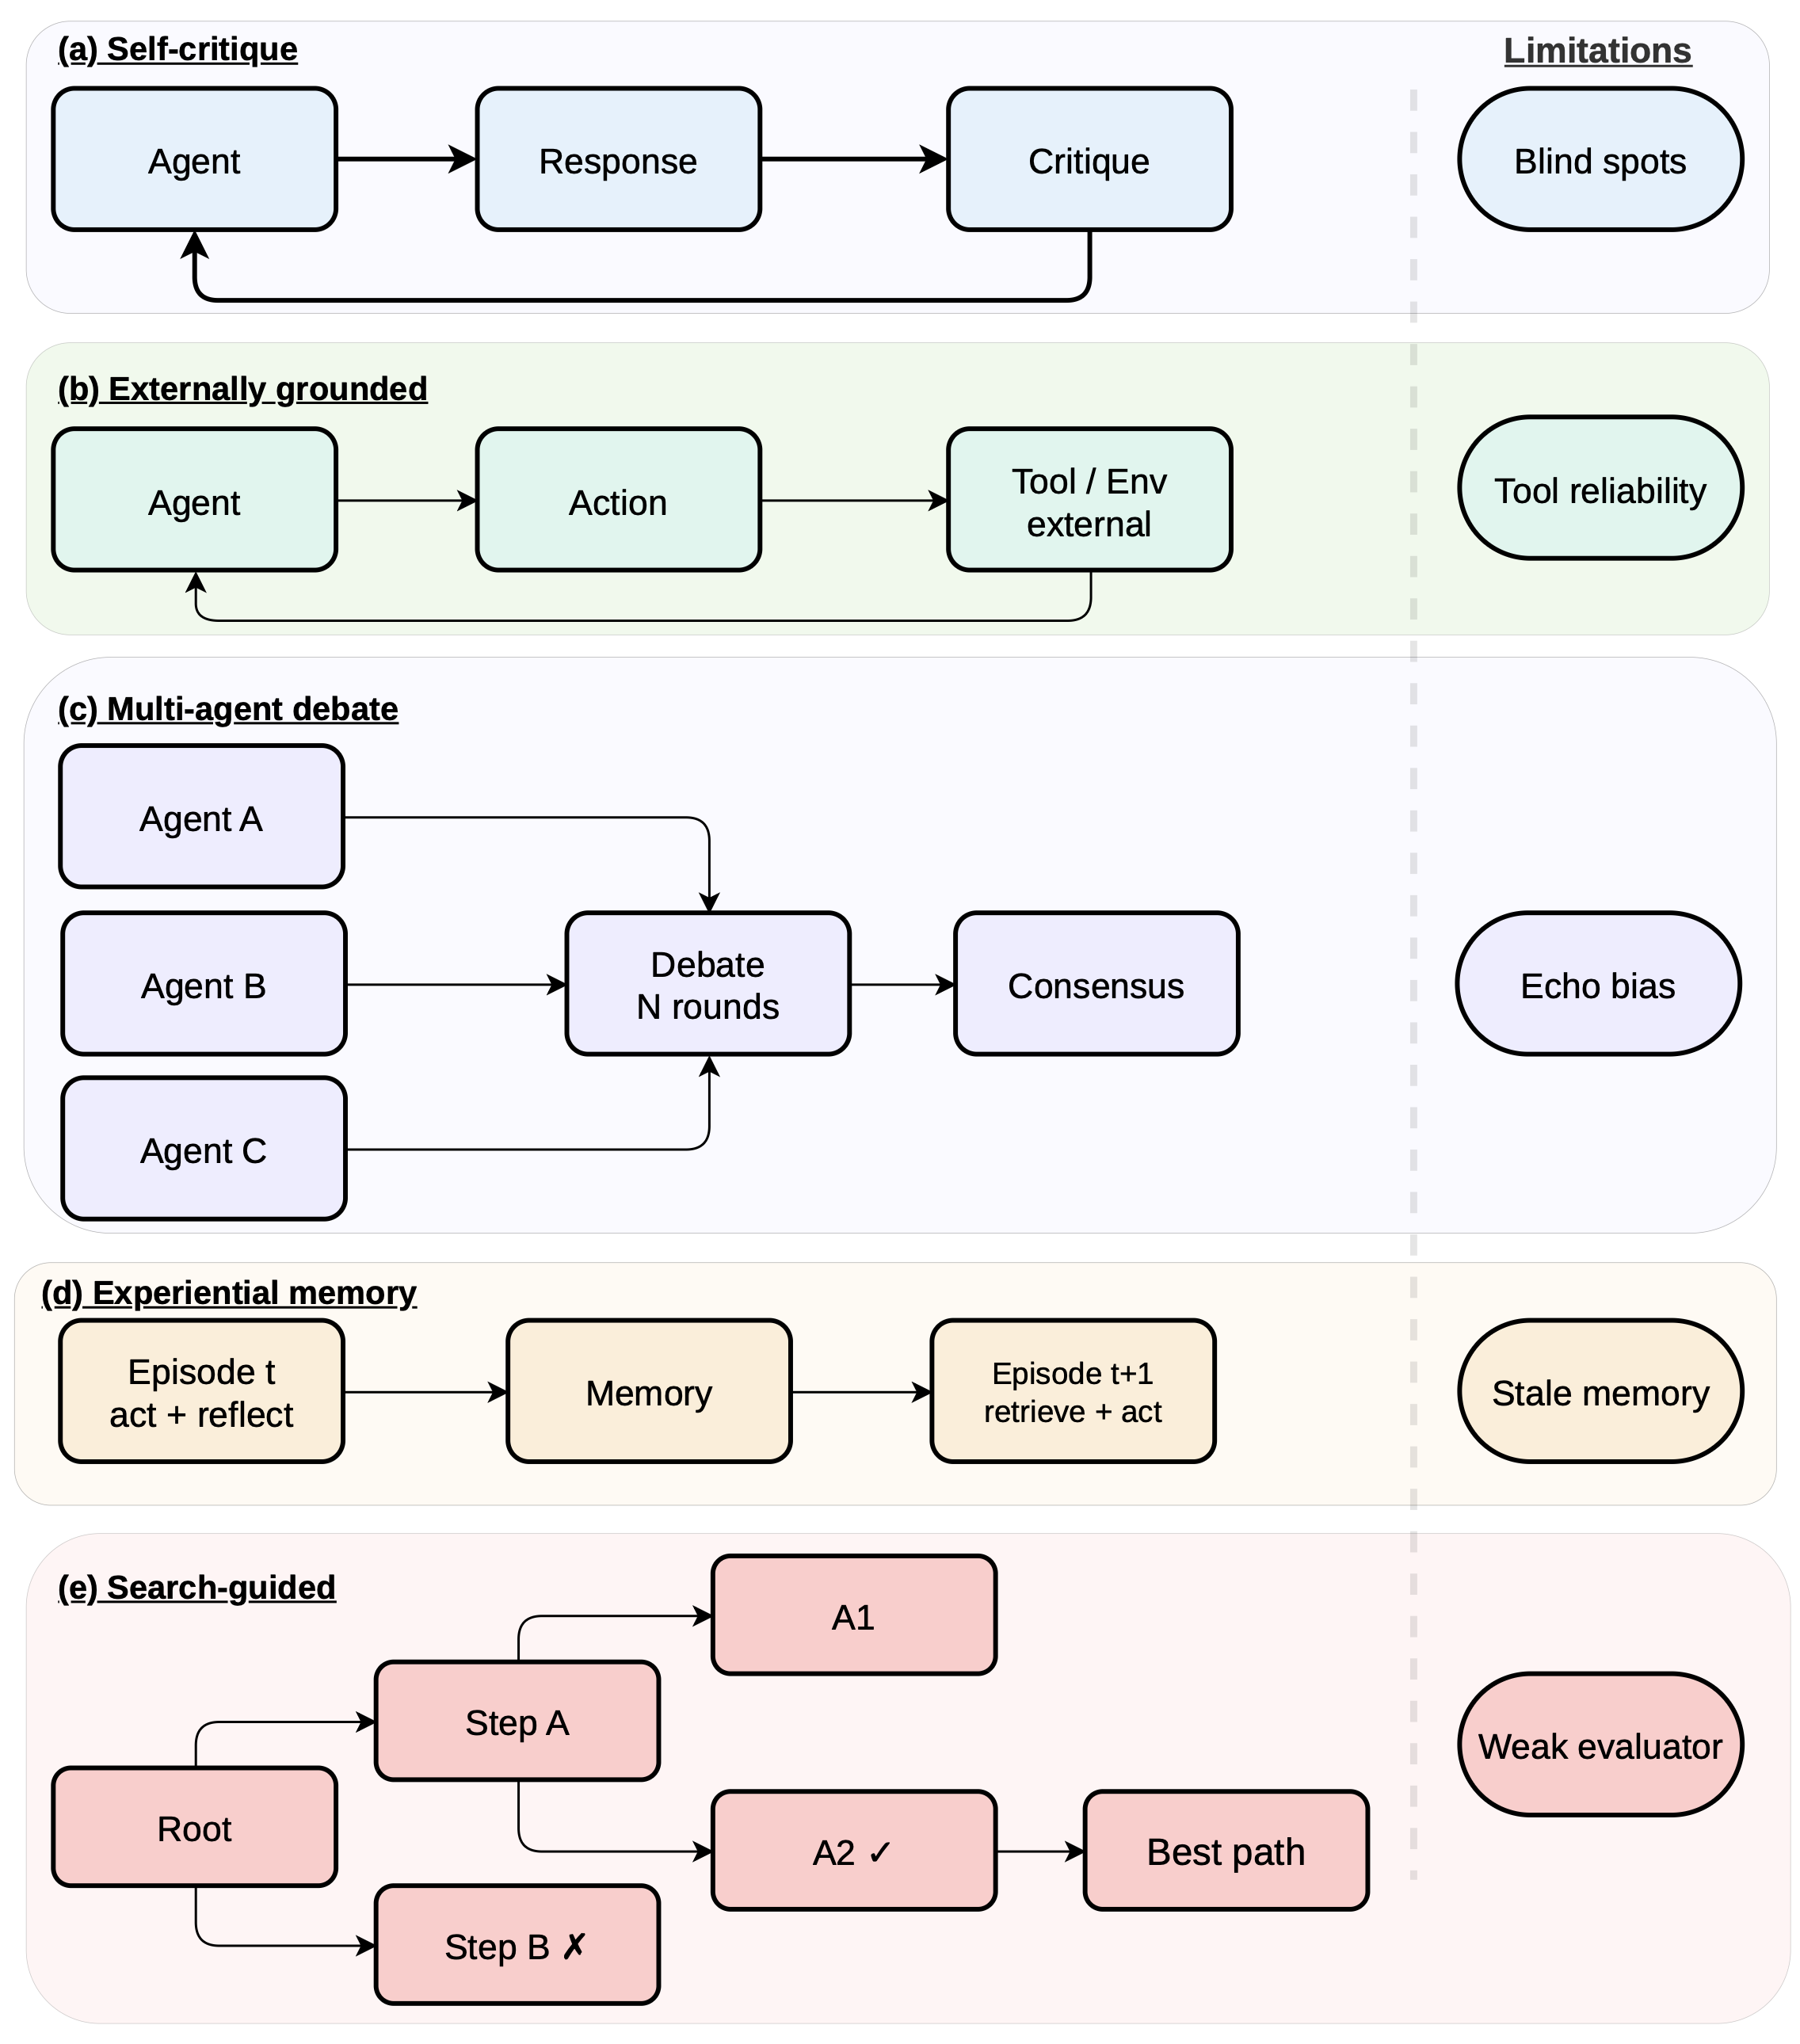
\includegraphics[width=1.05\linewidth]{paper_images/Figure-3-new.png}
    \caption{\footnotesize Inference-time verbal feedback mechanisms. Each subcategory exhibits a distinct feedback loop structure: (a) self-critique loops within a single model, (b) externally grounded critique incorporates verified tool or environment output, (c) multi-agent debate distributes critique across parallel model instances and converges to a refined output, (d) experiential memory persists lessons across episodes, and (e) search-guided deliberation explores and prunes multiple candidate paths.}
    \label{fig:inference_time}
\end{figure}

With the task grounded, we turn to methods that refine reasoning within a single episode without updating model parameters, closely aligning with test-time compute scaling \citep{snell2024scaling}. As illustrated in Figure~\ref{fig:inference_time}, five subcategories differ in where critique originates: the model itself (\S\ref{sec:self-refine}), external tools (\S\ref{sec:external-critique}), peer models (\S\ref{sec:multi-agent-critique}), past episodes (\S\ref{sec:experiential Memory}), or parallel search paths (\S\ref{sec:search-guided}).

% This pillar covers methods where verbal feedback improves reasoning during inference without updating model parameters, closely aligning with the idea of test-time compute scaling \citep{snell2024scaling}. As illustrated in Figure~\ref{fig:inference_time}, the five subcategories differ in where critique originates and how it feeds back: from the model itself (self-critique- \S\ref{sec:self-refine}), from external tools (grounded critique- \S\ref{sec:external-critique}), from peer models (debate- \S\ref{sec:multi-agent-critique}), from past episodes (memory- \S\ref{sec:experiential Memory}), or from parallel search paths (search guided deliberation - \S\ref{sec:search-guided}).


\subsection{Self-Critique}%
\label{sec:self-refine}
The simplest deliberative loop asks the model to critique its own output and revise accordingly. Self-Refine \citep{madaan2023selfrefine} formalized this pattern, building on Constitutional AI's \citep{bai2022constitutional} demonstration that models can evaluate outputs against written principles. The primary challenge is circularity. Replacing self-generated critique with evaluation from a separately trained critic enhances reasoning \citep{paul2024refiner}, which indicates that feedback quality is the main bottleneck. Self-correction degrades when the critique source shares the generator's blind spots \citep{huang2023large, kamoi2024can}, especially in smaller models \citep{olausson2024self}. Mitigation strategies include Socratic decomposition into verifiable steps \citep{shi2025ssr} and parallel self-refinement across candidates \citep{wang2025learning}. However, when errors arise from gaps in the model's knowledge, internal feedback mechanisms cannot identify the missing information.
 


\subsection{Externally Grounded Critique}%
\label{sec:external-critique}

External grounding addresses this circularity by anchoring verbal feedback in deterministic tool output \citep{schick2023toolformer}. Verified signals, such as execution traces, unit test verdicts, search results, and API responses \citep{chen2024teaching, gou2024toratoolintegratedreasoningagent}, facilitate the generation of corrected outputs \citep{gou2024critic, yang2024swe, wang2024executable}. Additionally, end-to-end reinforcement learning enables models to utilize such feedback more effectively \citep{gehring2024rlef}. The primary failure mode shifts from blind spots to trust asymmetry: the model receives accurate tool output but may misattribute the root cause of a reported trace. Practical limitations persist, including infrastructure overhead, poor scalability of latency, and the restriction of grounded critique to domains with a verifiable oracle.



\subsection{Multi-Agent Critique / Debate}%
\label{sec:multi-agent-critique}
Multi-agent debate distributes verbal critique across parallel model instances, frequently assigning distinct personas to enhance perspective \citep{hong2024metagpt}. The exchange of critiques can improve reasoning even among identical models \citep{du2023debate}, while the introduction of diverse roles further strengthens the quality of discussion \citep{chan2023chatevalbetterllmbasedevaluators}. Communication topology is a critical factor; full-broadcast designs incur substantial token overhead \citep{choi2026debate}, motivating the exploration of sparse alternatives \citep{li2024improving}. Models may also be trained specifically for debate, enabling them to revise reasoning in response to conflicting opinions \citep{liu2026learningselfdebatepreparingreasoning}. Adaptive heterogeneous frameworks have demonstrated improvements in mathematical reasoning \citep{zhou2025adaptive}. However, the primary limitation is that distributing critique is only effective when participating models are genuinely diverse. When models share biases, the process yields redundant consensus \citep{estornell2024multi, liang2024encouragingdivergentthinkinglarge}, and current debate methods do not consistently outperform simpler single-agent strategies \citep{choi2026debate}.


\subsection{Experiential Memory}%
\label{sec:experiential Memory}


Previous approaches regenerate feedback from scratch in each episode. In contrast, experiential memory distills reusable lessons into persistent storage, categorized as episodic (raw logs), semantic (distilled rules), and procedural (reusable skills) \citep{zhang2025survey}. \added{Although stored lessons persist across episodes, we classify memory by the moment of consumption: a retrieved lesson acts as deliberative feedback within the current episode, and Table~\ref{tab:hybrid} records the boundary with long-term adaptation.} Reflexion \citep{shinn2023reflexion} stores raw verbal feedback, ExpeL \citep{zhao2024expel} extracts insights from paired successes and failures, and Voyager \citep{wang2023voyager} accumulates executable skills. Recent surveys have formalized these mechanisms \citep{du2026memory}, while MemBench evaluates memory quality through downstream performance \citep{tan2025membench}. However, persisting feedback can also perpetuate errors: poor-quality memories propagate mistakes, expanding memory stores require complex retrieval \citep{park2023genagents}, outdated knowledge can mislead in non-stationary environments \citep{zhang2025survey}, and adversarial injection may induce cross-session drift \citep{dong2026memory}.





\subsection{\texorpdfstring{\removed{Search-Guided Deliberation}\added{Evaluator Feedback in Search}}{Evaluator Feedback in Search}}%
\label{sec:search-guided}
\added{The inclusion criterion for this subcategory is the verbal evaluator signal consumed during search, not the search procedure itself; decoding strategies that involve no linguistic feedback fall outside VRL.} While previous approaches refine a single trajectory, \removed{search-guided deliberation}\added{these methods} explore\removed{s} multiple candidate paths and employ\removed{s} verbal feedback to determine which paths to expand, prune, or abandon \citep{wang-etal-2025-dont}. The Tree of Thoughts framework \citep{yao2023tree} samples several intermediate thoughts and evaluates them through self-assessment, thereby extending chain-of-thought prompting \citep{wei2022chain} with a tree-based search mechanism. Reasoning via Planning \citep{hao2023reasoning} and Graph of Thoughts \citep{besta2024graph} further generalize the underlying topology, permitting non-linear dependencies such as aggregation and refinement. A key advantage of these methods is that verbal feedback can be applied at every thought level, which facilitates earlier identification of unproductive paths. However, exploring multiple states necessitates numerous large language model (LLM) calls, rendering these methods considerably more expensive than single-pass generation \citep{xie2023self}.




